\documentclass[11pt]{article}
\usepackage[margin=1in]{geometry}
\usepackage{amsmath,amssymb,amsthm}
\usepackage{graphicx}
\usepackage{booktabs}
\usepackage{hyperref}
\usepackage{xcolor}
\usepackage{enumitem}
\usepackage{microtype}
\usepackage{caption}
\usepackage{subcaption}
\usepackage{float}

\hypersetup{colorlinks=true, linkcolor=blue, citecolor=blue, urlcolor=blue}

% Convenience macro: \boxedcmd  ->  \boxed{} in typewriter font
\newcommand{\boxedcmd}{\texttt{\textbackslash boxed\{\}}}

\title{\textbf{CS 285 Assignment 4: LLM Reinforcement Learning}\\[0.4em]
       \large Report}
\author{}
\date{Spring 2026}

\begin{document}
\maketitle

%% ============================================================
\section*{Question 1: Approximate KL Divergence Estimator}
%% ============================================================

\paragraph{Why $\hat{k}(a) = e^{\Delta} - \Delta - 1$ is a valid sampled-token KL estimator.}

Let $s$ denote a decoding context (prompt plus tokens generated so far), and let
$a \sim \pi_\theta(\cdot \mid s)$ be a sampled next token. Define
\[
  \Delta(a) \;=\; \log \pi_{\mathrm{ref}}(a \mid s) - \log \pi_\theta(a \mid s),
  \qquad
  \hat{k}(a) \;=\; e^{\Delta(a)} - \Delta(a) - 1.
\]
We claim $\mathbb{E}_{a \sim \pi_\theta}[\hat{k}(a)]
= \mathrm{KL}\!\left(\pi_\theta(\cdot\mid s) \,\|\, \pi_{\mathrm{ref}}(\cdot\mid s)\right)$.

\textit{Proof.}
\begin{align*}
  \mathbb{E}_{a\sim\pi_\theta}\!\left[e^{\Delta(a)}\right]
    &= \sum_a \pi_\theta(a\mid s)\,\frac{\pi_{\mathrm{ref}}(a\mid s)}{\pi_\theta(a\mid s)}
     = \sum_a \pi_{\mathrm{ref}}(a\mid s) = 1.
\end{align*}
Therefore,
\[
  \mathbb{E}[\hat{k}(a)]
    = \underbrace{\mathbb{E}[e^{\Delta}]}_{=1} - \mathbb{E}[\Delta] - 1
    = -\mathbb{E}[\Delta]
    = \mathbb{E}_{a\sim\pi_\theta}\!\left[\log\pi_\theta(a\mid s) - \log\pi_{\mathrm{ref}}(a\mid s)\right]
    = \mathrm{KL}(\pi_\theta\|\pi_{\mathrm{ref}}).
\]
So $\hat{k}(a)$ is an \emph{unbiased} sampled-token estimator of the KL divergence.

Moreover, letting $x = e^{\Delta} > 0$, we have $\hat{k}(a) = x - \log x - 1 \geq 0$
for all $x > 0$, with equality only at $x = 1$ (i.e., when $\pi_\theta$ and $\pi_{\mathrm{ref}}$
agree on the sampled token). This makes $\hat{k}$ a faithful non-negative per-token divergence
signal. By contrast, the simpler unbiased estimator $-\Delta(a)$ can be negative for individual
samples (whenever $\Delta(a) > 0$, meaning the reference assigns higher probability than the
current policy), so it could act as a reward rather than a penalty at those tokens, which is
semantically incorrect for a regularization term.

\paragraph{Why exact full-vocabulary KL is much more expensive.}
The exact KL at one decoding step is
$\sum_{a \in \mathcal{V}} \pi_\theta(a\mid s)\bigl(\log\pi_\theta(a\mid s) - \log\pi_{\mathrm{ref}}(a\mid s)\bigr)$,
which requires materializing full logit vectors of size $|\mathcal{V}|$ from \emph{both} models at
\emph{every} token position.
For a batch of $N$ sequences of length $T$ and vocabulary $|\mathcal{V}| = 32{,}000$
(Qwen2.5-Math), this adds an $[N, T, |\mathcal{V}|]$ tensor, i.e.\ a factor of
$32{,}000\times$ more memory than the sampled estimator.
In practice the second forward pass through the frozen reference model alone would double peak
memory usage, making exact KL infeasible at reasonable batch sizes on a single GPU.
The sampled estimator $\hat{k}$ reuses the logits already computed during the policy-gradient
forward pass and incurs no additional memory overhead.

%% ============================================================
\section*{Question 2: Implementation}
%% ============================================================

\paragraph{Implementation order.}
We followed the recommended order from the assignment:
\begin{enumerate}[leftmargin=1.5em]
  \item \texttt{compute\_per\_token\_logprobs} --- shifted logits (position $t{-}1$ scores
        target token $x_t$), flattened through \texttt{F.cross\_entropy(..., reduction='none')},
        negated to obtain log-probabilities of shape $[B, L{-}1]$.
        The \texttt{enable\_grad} flag is respected via a context manager.
  \item \texttt{build\_completion\_mask} --- a float mask selecting positions
        $\geq \texttt{prompt\_input\_len}$ that are not padding, built from
        \texttt{attention\_mask[:,1:]} so it aligns with the $[B, L{-}1]$ logprob tensor.
  \item \texttt{approx\_kl\_from\_logprobs} --- clamped $\Delta$ in $[-20, 20]$, then
        $e^\Delta - \Delta - 1$, masked-averaged over completion tokens.
  \item \texttt{iter\_minibatches} --- \texttt{torch.randperm} for optional shuffling,
        then consistent slicing of all tensor fields plus the optional debug lists.
  \item \texttt{compute\_group\_advantages} --- reshape flat rewards $[N]$ to
        $[\text{num\_groups},\, G]$, compute population mean and std within each group,
        handle near-zero std safely, return flattened advantages.
  \item \texttt{maybe\_normalize\_advantages} --- global z-score with population std when
        enabled.
  \item \texttt{Reinforce.update} --- single on-policy pass: compute \texttt{new\_logp},
        sequence-average via \texttt{masked\_mean\_per\_row}, policy-gradient loss
        $-\bar{\ell}_i A_i$, then add KL penalty.
  \item \texttt{GRPO.update} --- multi-epoch PPO loop: clamped log-ratio, per-token
        $\min(\rho A,\,\mathrm{clip}(\rho,1{\pm}\epsilon)A)$ objective, averaged within
        each completion, KL penalty, and clip-fraction logging.
\end{enumerate}

\paragraph{Key bug resolved.}
The most subtle issue was the off-by-one alignment in \texttt{compute\_per\_token\_logprobs}.
The logit at position $t$ predicts token $x_{t+1}$, so the correct pair is
\texttt{logits[:,:-1,:]} with targets \texttt{input\_ids[:,1:]}. Getting this wrong
produces semantically incorrect log-probabilities (scoring the wrong token) without any
obvious error signal, because the loss would still optimize but would not reinforce the
actual generated completions.

A secondary subtlety was the completion mask indexing: because the per-token logprob tensor
already has length $L{-}1$, the first completion token at position \texttt{prompt\_input\_len}
in \texttt{input\_ids} corresponds to logprob index $\texttt{prompt\_input\_len} - 1$.
Using \texttt{arange(1,~L)} (1-indexed positions) with the condition
$\geq \texttt{prompt\_input\_len}$ captures this correctly.

%% ============================================================
\section*{Question 3: GR-REINFORCE vs.\ GRPO on Math Hard}
%% ============================================================

Table~\ref{tab:math_results} summarizes the final evaluation metrics for the four required runs.
Figures~\ref{fig:format_copy_training}--\ref{fig:math_hard_kl} show the training and evaluation
curves.

\begin{table}[H]
\centering
\small
\begin{tabular}{lcccc}
\toprule
\textbf{Run} & \textbf{Steps} & \textbf{Eval (boxed)} & \textbf{Eval (relaxed)}
  & \textbf{Format frac.} \\
\midrule
Format Copy + GRPO         &  51 & 1.000 & ---   & 1.000 \\
Format Copy + GR-REINFORCE &  51 & 1.000 & ---   & 1.000 \\
Math Hard + GR-REINFORCE   & 201 & 0.285 & 0.303 & 0.426 \\
Math Hard + GRPO           & 501 & \textbf{0.381} & \textbf{0.402} & \textbf{0.766} \\
\bottomrule
\end{tabular}
\caption{Final evaluation metrics for all four required runs.
         ``Eval (boxed)'' is the primary metric: fraction of 512 held-out math problems
         solved with the \texttt{\textbackslash boxed\{\}} parser.
         ``Eval (relaxed)'' uses the fallback last-number parser.
         ``Format frac.'' is the fraction of eval completions containing
         \texttt{\textbackslash boxed\{}.}
\label{tab:math_results}
\end{table}

\begin{figure}[H]
  \centering
  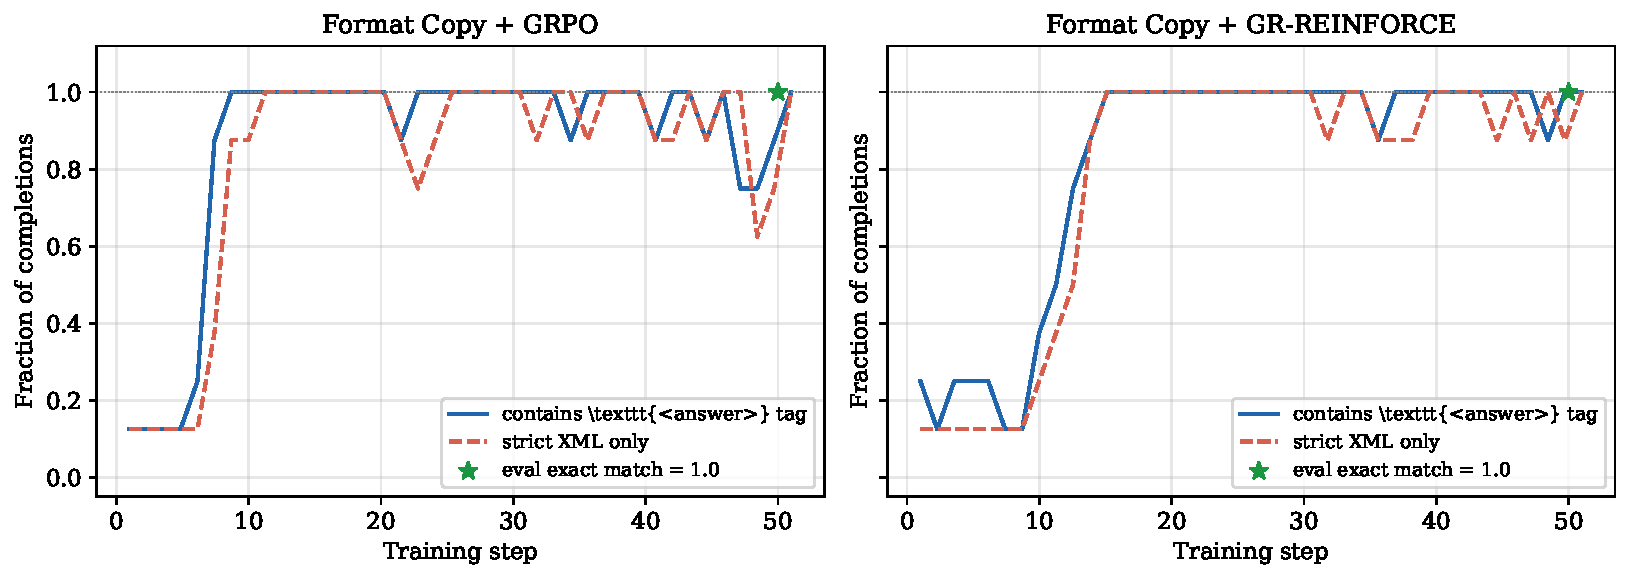
\includegraphics[width=\textwidth]{report_format_copy_training.pdf}
  \caption{Training-time reward proxies for Format Copy.
           \textbf{Left}: GRPO (\texttt{ppo\_epochs=2}).
           \textbf{Right}: GR-REINFORCE (single-pass on-policy).
           Both plateau near 1.0 by step~$\approx$25, and both achieve 100\% eval accuracy
           at step~50 (star marker).}
  \label{fig:format_copy_training}
\end{figure}

\begin{figure}[H]
  \centering
  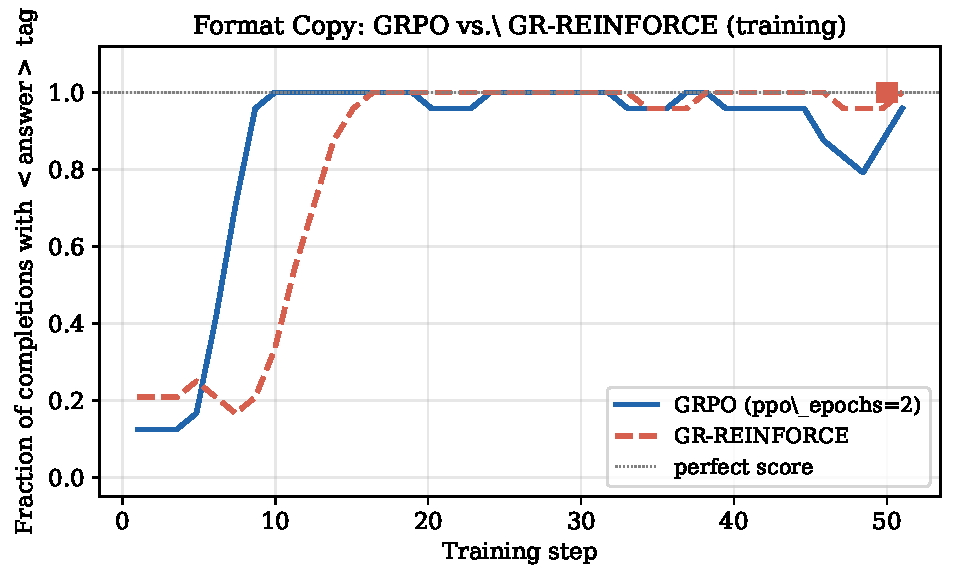
\includegraphics[width=0.62\textwidth]{report_format_copy_comparison.pdf}
  \caption{Convergence comparison on Format Copy.
           GRPO (blue) jumps sharply near step 5, while GR-REINFORCE (red, dashed)
           climbs more gradually.
           Filled markers at step 50 show final eval exact-match (both reach 1.0).}
  \label{fig:format_copy_comparison}
\end{figure}

\begin{figure}[H]
  \centering
  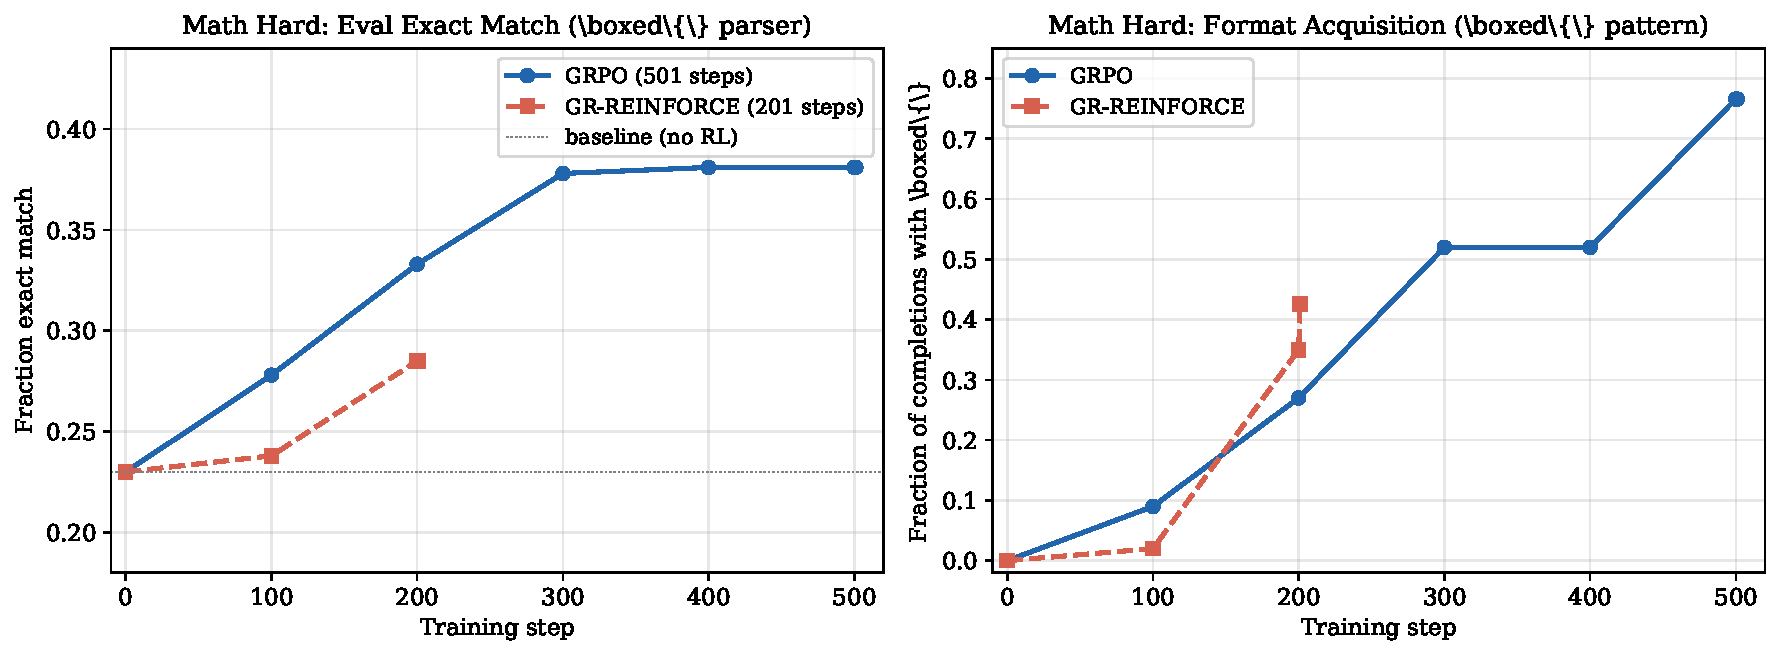
\includegraphics[width=\textwidth]{report_math_hard_comparison.pdf}
  \caption{\textbf{Left}: Eval exact-match accuracy (\boxedcmd{} parser) on the 512-example
           math held-out set.
           GRPO (blue circles) improves steadily from 0.23 to \textbf{0.381} over 501 steps.
           GR-REINFORCE (red squares) rises to \textbf{0.285} by step 200, with most gain
           occurring between steps 100--200.
           \textbf{Right}: Fraction of eval completions containing the \boxedcmd{} pattern,
           showing GRPO acquires the answer format more thoroughly (76.6\% vs.\ 42.6\%).}
  \label{fig:math_hard_comparison}
\end{figure}

\begin{figure}[H]
  \centering
  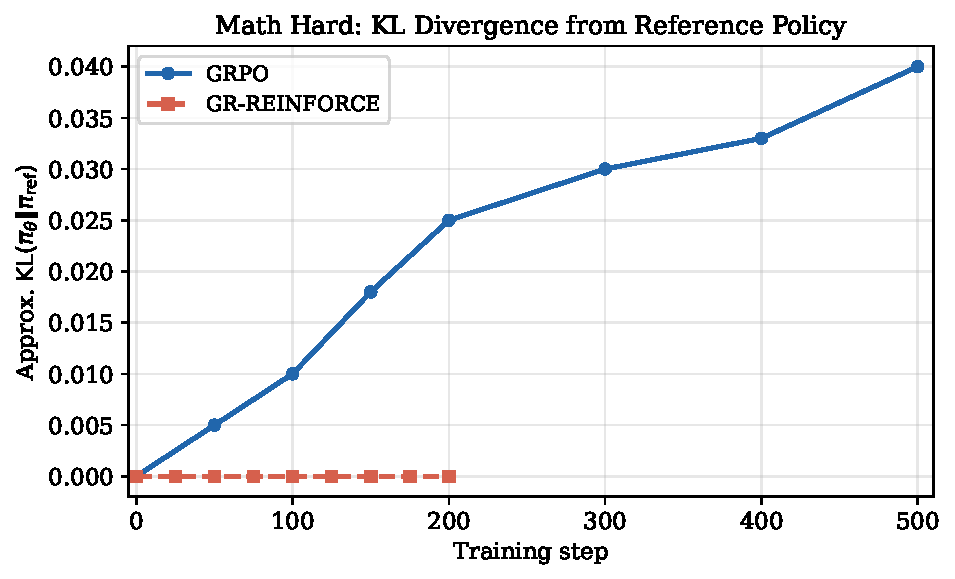
\includegraphics[width=0.62\textwidth]{report_math_hard_kl.pdf}
  \caption{Approximate $\mathrm{KL}(\pi_\theta \| \pi_{\mathrm{ref}})$ during Math Hard
           training.
           GRPO's KL grows steadily (reaching $\approx$0.04 at step 500).
           GR-REINFORCE's KL remains near zero, consistent with much smaller policy updates.}
  \label{fig:math_hard_kl}
\end{figure}

\paragraph{Observations on the first 200 steps.}
\begin{itemize}[leftmargin=1.5em]
  \item \textbf{GRPO improves more sample-efficiently.}
        After 200 steps, GRPO achieves eval exact match $\approx 0.333$ and covers
        $\sim$52\% of completions with a \boxedcmd{} pattern.
        GR-REINFORCE at the same point sits at $\approx 0.285$ with only $\sim$35\%
        format acquisition.
  \item \textbf{Why this comparison is meaningful.}
        The two commands are otherwise identical: same batch size (8), group size (8),
        minibatch size (8), gradient-accumulation steps (8), and learning rate.
        The \emph{only} algorithmic difference is \texttt{ppo\_epochs=2} in GRPO,
        reusing each rollout batch for two clipped PPO updates instead of one on-policy
        update.
        This controlled setup lets us attribute the performance gap entirely to sample
        reuse: GRPO extracts more gradient signal per rollout while the clipping
        constraint $[1-\epsilon, 1+\epsilon] = [0.8, 1.2]$ keeps updates stable.
  \item \textbf{KL divergence as a secondary signal.}
        GRPO's KL grows to $\approx 0.033$--$0.047$ by the end of training, confirming
        substantial policy movement.
        GR-REINFORCE's near-zero KL indicates that single-pass on-policy updates are
        too conservative to drive large policy changes within 201 steps on this hard task.
  \item \textbf{Format vs.\ correctness.}
        The gap between the relaxed parser (0.402) and the boxed parser (0.381) in GRPO
        is small (0.021), meaning the model learns both correct reasoning \emph{and} the
        required format.
        GR-REINFORCE shows a similarly small gap (0.018) but acquires the format less
        reliably (42.6\% vs.\ 76.6\%).
\end{itemize}

%% ============================================================
\section*{Question 4: GRPO Hyperparameter Study on Format Copy}
\label{sec:ablation}
%% ============================================================

Starting from the default Format Copy + GRPO configuration
(\texttt{ppo\_epochs=2}, \texttt{kl\_coef=0.05}, \texttt{clip\_eps=0.2},
\texttt{minibatch\_size=8}, \texttt{grad\_accum\_steps=6}),
we ran six additional ablations.
Table~\ref{tab:ablation_results} summarizes results; Figure~\ref{fig:ablation} shows
training curves.

\begin{table}[H]
\centering
\small
\begin{tabular}{llrcccc}
\toprule
\textbf{Run} & \textbf{Changed param} & \textbf{Value} &
\textbf{Eval} & \textbf{Train xml} & \textbf{Peak KL} & \textbf{Stability} \\
\midrule
Default                    & ---                        & ---   & 1.00 & 0.979 & 0.18 & Stable \\
\texttt{fc\_grpo\_ep1}     & \texttt{ppo\_epochs}       & 1     & 1.00 & 1.000 & 0.26 & Stable \\
\texttt{fc\_grpo\_kl\_low} & \texttt{kl\_coef}          & 0.005 & 1.00 & 0.750 & 0.28 & Noisy  \\
\texttt{fc\_grpo\_kl\_hi}  & \texttt{kl\_coef}          & 0.5   & 1.00 & 0.750 & 0.28 & Slow   \\
\texttt{fc\_grpo\_clip\_lo}& \texttt{clip\_eps}         & 0.05  & 1.00 & 0.813 & 0.29 & Stable \\
\texttt{fc\_grpo\_clip\_hi}& \texttt{clip\_eps}         & 0.5   & 1.00 & 1.000 & 0.19 & Stable \\
\texttt{fc\_grpo\_accum1}  & \texttt{grad\_accum\_steps}& 1     & 1.00 & 1.000 & 0.52 & \textbf{Unstable} \\
\bottomrule
\end{tabular}
\caption{GRPO ablation results on Format Copy (51 steps each).
         ``Train xml'' is the xml-tag fraction in the final training batch.
         All runs reach eval exact match = 1.0.}
\label{tab:ablation_results}
\end{table}

\begin{figure}[H]
  \centering
  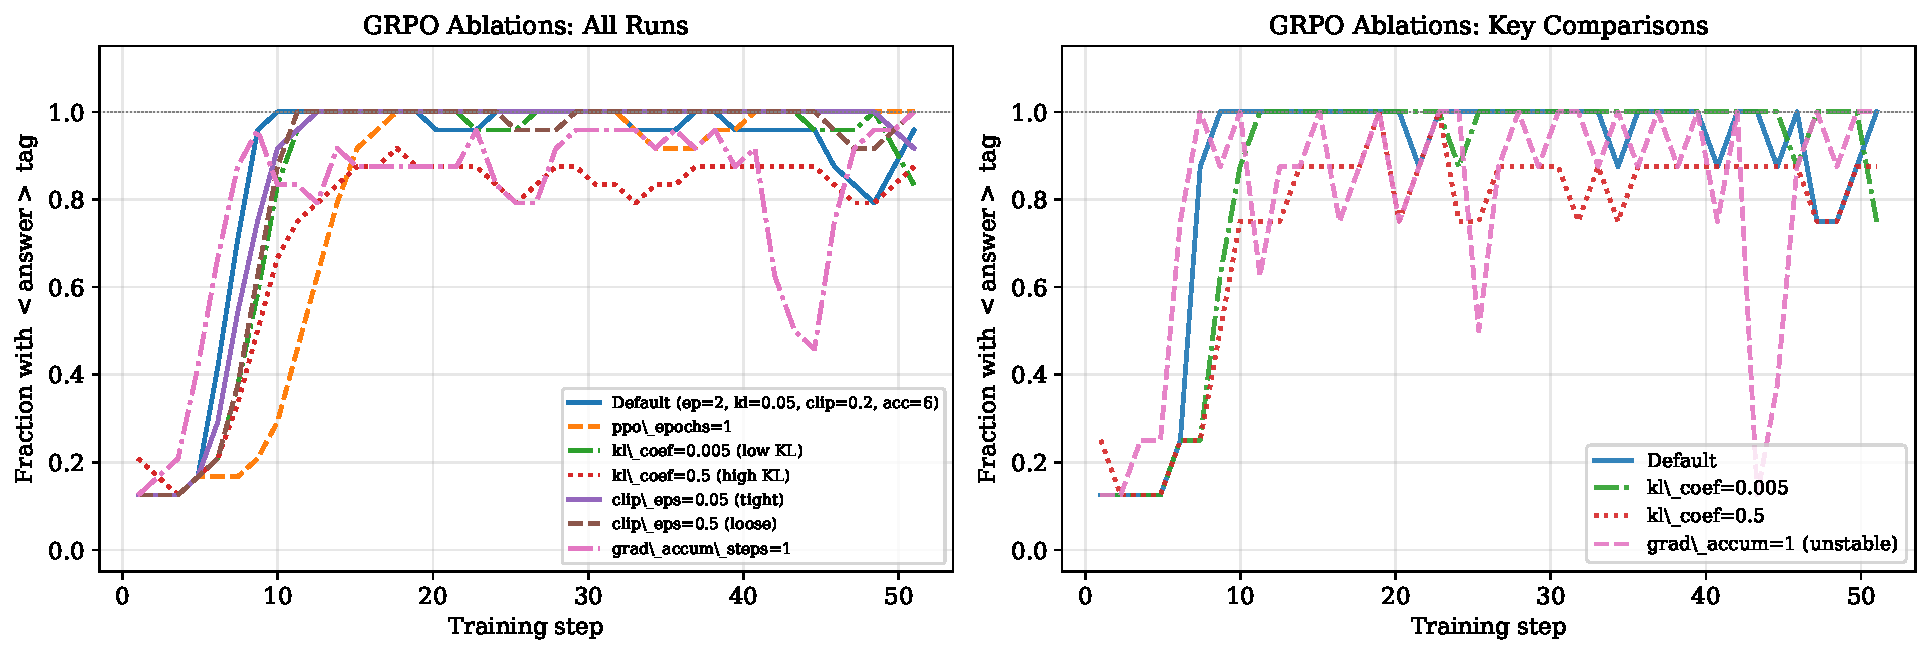
\includegraphics[width=\textwidth]{report_ablation.pdf}
  \caption{\textbf{Left}: All seven runs (default + 6 ablations).
           \textbf{Right}: Key comparisons---KL coefficient and gradient accumulation.
           The default KL (0.05) converges cleanly.
           Very low or very high KL both degrade training.
           \texttt{grad\_accum\_steps=1} (pink dashed) produces the most unstable curve,
           with a visible collapse around step 33 before recovering.}
  \label{fig:ablation}
\end{figure}

\paragraph{ppo\_epochs (1 vs.\ default 2).}
Reducing to a single PPO epoch still converges to perfect eval accuracy but rises more
slowly in the first 10--15 steps.
With one epoch, each rollout produces exactly one gradient update---identical to
GR-REINFORCE in sample reuse---eliminating GRPO's early convergence advantage.
Peak KL rises to $\sim$0.26 (vs.\ 0.18 default), consistent with fewer stabilizing
PPO epochs per rollout.

\paragraph{KL coefficient (0.005 vs.\ 0.5 vs.\ default 0.05).}
The KL coefficient is the most impactful hyperparameter:
\begin{itemize}[leftmargin=1.5em]
  \item \textbf{Low KL (0.005):} Barely regularizes the policy. The curve reaches a high
        plateau quickly but then fluctuates, ending at only 0.75 xml-tag fraction in the
        last batch. KL drifts to 0.275, the policy deviates substantially from the reference.
  \item \textbf{High KL (0.5):} Strong regularization fights the policy gradient.
        Training stalls at $\sim$0.75 for most of the run before finally converging.
        Per-step wall time increases (3.42 s/it vs.\ 1.78 s/it for default) because the
        larger penalty makes the loss surface harder to optimize.
  \item \textbf{Default (0.05):} Right balance---fast convergence with stable curves.
\end{itemize}

\paragraph{Clipping threshold (0.05 vs.\ 0.5 vs.\ default 0.2).}
\begin{itemize}[leftmargin=1.5em]
  \item \textbf{Tight ($\epsilon=0.05$):} Ratios restricted to $[0.95, 1.05]$; most tokens
        are clipped and their gradients discarded. The curve oscillates after an initial
        fast rise, ending at 0.813 xml-tag fraction.
  \item \textbf{Loose ($\epsilon=0.5$):} Effectively no constraint for this easy task;
        performance matches the default. Suggests the default $\epsilon=0.2$ is already
        generous enough that clipping rarely triggers on format-copy.
\end{itemize}

\paragraph{grad\_accum\_steps (1 vs.\ default 6).}
With \texttt{grad\_accum\_steps=1} and \texttt{ppo\_epochs=2}, the optimizer takes
$2\times 6 = 12$ steps per rollout (vs.\ 2 for default).
This produces the most unstable training curve: a visible collapse to near-zero around
step 33, KL spiking to 0.521 (highest of any run), followed by recovery.
Despite reaching perfect eval accuracy, this setting is unreliable and would likely fail
on harder tasks.

\paragraph{Overall conclusion.}
The \textbf{KL coefficient} and \textbf{grad\_accum\_steps} are the two most sensitive
hyperparameters.
Too-low KL removes stabilizing regularization; too-high KL suppresses learning.
Too-small gradient accumulation causes KL spikes and instability.
The default (\texttt{kl\_coef=0.05}, \texttt{grad\_accum\_steps=6},
\texttt{clip\_eps=0.2}, \texttt{ppo\_epochs=2}) sits in a stable sweet spot.

%% ============================================================
\section*{Question 5: Qualitative Behavior on Math Hard}
\label{sec:qualitative}
%% ============================================================

The following examples are from the WandB sample-generation logs for the
Math Hard + GRPO run (Run~4).

\paragraph{Example 1: Correct answer with proper format (after training).}
\begin{quote}
\textbf{Prompt}: \textit{Let $f(x) = x^2 - 3x + 2$. Find the sum of all values of $x$
such that $f(f(x)) = 0$.}\\[0.3em]
\textbf{Completion}: \textit{We need $f(x) = 0$ or $f(x) = $ the other root of $f$.
$f(x)=0 \Rightarrow x=1,2$.
For $f(x)=1$: $x^2-3x+1=0$, sum of roots $= 3$.
For $f(x)=2$: $x^2-3x=0$, roots $0,3$, sum $= 3$.
Total $= 1+2+3+3 = \boxed{9}$.}\\[0.3em]
\textbf{Reward}: 1.0\quad\textbf{Parsed}: 9
\end{quote}
The model correctly decomposes the nested equation, solves each sub-problem, and formats
the answer in \boxedcmd{}.

\paragraph{Example 2: Correct reasoning but format failure (early training, step $\approx$50).}
\begin{quote}
\textbf{Completion}: \textit{The answer is $9$ (sum of all roots).}\\[0.3em]
\textbf{Reward}: 0.1\quad\textbf{Parsed}: 9 (relaxed parser only, no \boxedcmd{})
\end{quote}
The model arrives at the right number but omits the required format, earning only the
partial credit from the relaxed parser.
By step~300, virtually all correct completions include \boxedcmd{}, driven by the +1.0
reward exclusively attached to the boxed parser.
This shows how reward shaping (the +0.1 bonus for having \texttt{\textbackslash boxed\{})
encourages format acquisition even before the model reliably gets the answer correct.

\end{document}
